% -*- latex -*-
%%%%%%%%%%%%%%%%%%%%%%%%%%%%%%%%%%%%%%%%%%%%%%%%%%%%%%%%%%%%%%%%
%%%%%%%%%%%%%%%%%%%%%%%%%%%%%%%%%%%%%%%%%%%%%%%%%%%%%%%%%%%%%%%%
%%%%
%%%% This text file is part of the lecture slides for
%%%% `Parallel Programming in MPI and OpenMP'
%%%% by Victor Eijkhout, copyright 2012-2024 
%%%%
%%%% Sync-slides.tex : slides about OpenMP workshare constructs
%%%%
%%%%%%%%%%%%%%%%%%%%%%%%%%%%%%%%%%%%%%%%%%%%%%%%%%%%%%%%%%%%%%%%
%%%%%%%%%%%%%%%%%%%%%%%%%%%%%%%%%%%%%%%%%%%%%%%%%%%%%%%%%%%%%%%%

\begin{numberedframe}{Need for synchronization}
  \begin{itemize}
  \item The loop and sections directives do not specify an ordering,\\
    sometimes you want to force an ordering.
  \item Barriers: global synchronization.
  \item Critical sections: only one process can execute a statement\\
    this prevents race conditions.
  \item Locks: protect data items from being accessed.
  \end{itemize}
\end{numberedframe}

\begin{numberedframe}{Barriers}
\small
  \begin{itemize}
  \item Every workshare construct has an implicit barrier:
\begin{verbatim}
#pragma omp parallel
{
  #pragma omp for
    for ( .. i .. )
      x[i] = ...
  #pragma omp for
    for ( .. i .. )
      y[i] = .. x[i] .. x[i+1] .. x[i-1] ...
}
\end{verbatim}
First loop is completely finished before second.
\item Explicit barrier:
\begin{verbatim}
#pragma omp parallel
{
  x = f();
#pragma omp barrier
  .... x ...
}
\end{verbatim}
  \end{itemize}
\end{numberedframe}

\begin{numberedframe}{Critical sections}
\begin{itemize}
  \item Critical section: One update at a time.
\begin{verbatim}
#pragma omp parallel
{
  double x = f();
#pragma omp critical
  global_update(x);
}
\end{verbatim}
\item \indextermtt{atomic} : special case for simple operations, possible
  hardware support
\begin{verbatim}
#pragma omp atomic
  t += x;
\end{verbatim}
\end{itemize}
\end{numberedframe}

\begin{numberedframe}{Warning}
  \begin{itemize}
  \item Critical sections are not cheap! The operating system takes
    thousands of cycles to coordinate the threads.
  \item Use only if minor amount of work.
  \item Do not use if a reduction suffices.
  \item Name your critical sections.
  \item Explore locks if there may not be a data conflict.
  \end{itemize}
\end{numberedframe}

\begin{numberedframe}{Critical sections and idle time}
    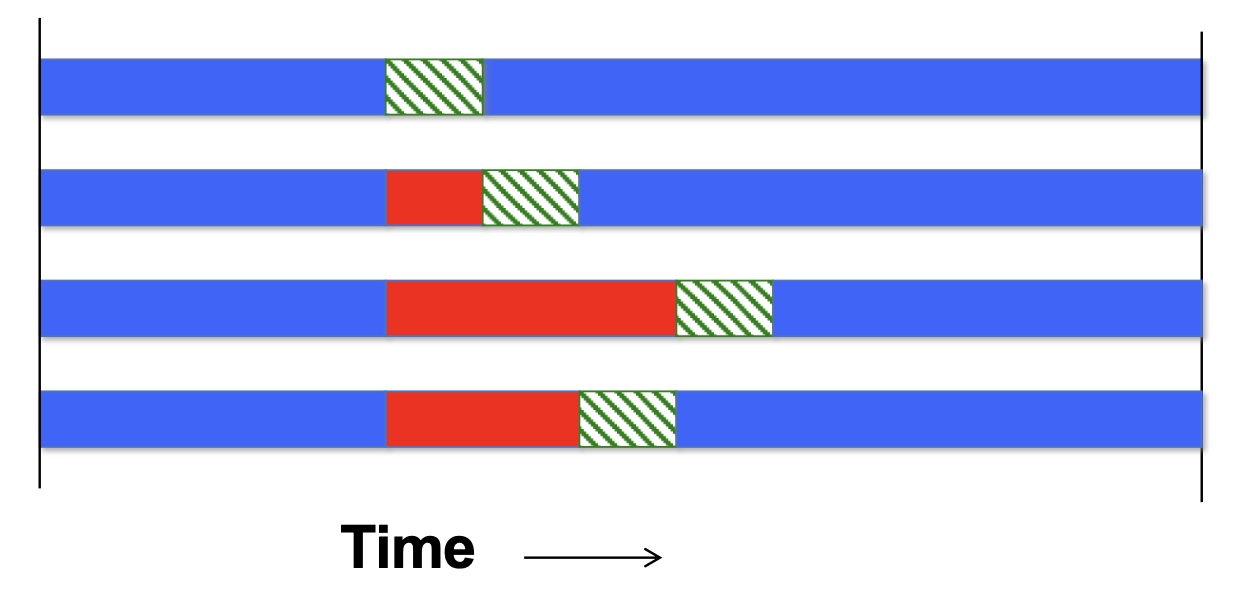
\includegraphics[scale=.5]{omp-idle}
    In effect, the execution becomes sequential!
\end{numberedframe}

\begin{numberedframe}{Do not misuse critical sections}
\begin{lstlisting}
#pragma omp parallel for
for ( /* i in whatever */ ) {
  #pragma omp critical
  s += /* expression with i */
}
\end{lstlisting}
  \begin{itemize}
  \item Use reduction if appropriate
  \item Only use if the enough other work in the iteration
  \end{itemize}
\end{numberedframe}

\begin{numberedframe}{Locks}
  \begin{itemize}
  \item Critical sections are coarse:\\
    they dictate exclusive acces to a \emph{statement}
  \item     Suppose you update a big table\\
    updates to non-conflicting locations should be allowed
  \item Locks protect a single data item.
  \end{itemize}
\end{numberedframe}

\begin{numberedframe}{Lock create and destoy}
  \begin{itemize}
  \item Variable to hold lock
  \item Create/destroy actual lock
  \end{itemize}
\cverbatimsnippet{lockinit}
\end{numberedframe}

\begin{numberedframe}{Use of lock}
  \begin{itemize}
  \item Same thread sets/unsets lock
  \item While lock is set, other threadds can not pass
  \end{itemize}
\cverbatimsnippet{lockupdate}
\end{numberedframe}

\begin{numberedframe}{Exercise: histogram}
  Basic idea:
\begin{lstlisting}
for ( i /* lots of cases */ )
  bin[ property(i) ]++;
\end{lstlisting}
Without a specific application, we let the bin number
be random:
\cverbatimsnippet{histobasic}
\end{numberedframe}

\begin{numberedframe}{Histogram 2}
  \begin{itemize}
  \item Make this omp parallel
  \item Observe that the result is not correct.
  \item   Experiment with number of threads and bins.
  \end{itemize}
\end{numberedframe}

\begin{numberedframe}{Histogram 3}
  \begin{itemize}
  \item Solve with histogram
  \item Experiment with number of threads and bins.
  \end{itemize}
\end{numberedframe}

\begin{numberedframe}{Histogram 3}
  \begin{itemize}
  \item Solve with locks\\
    (How many locks are needed?)
  \item Experiment with number of threads and bins.
  \end{itemize}
\end{numberedframe}

\endinput

\begin{numberedframe}{}
  \begin{itemize}
  \item 
  \end{itemize}
\end{numberedframe}

